\documentclass[10pt,a4paper]{article}
\usepackage[utf8]{inputenc}

% Define the page margin
\usepackage[margin=3cm]{geometry}

% Better typography (font rendering)
\usepackage{microtype}

% Math environments and macros
\usepackage{amsmath}
\usepackage{amsfonts}
\usepackage{amssymb}
\usepackage{amsthm}

% Define \includegraphics to include graphics
\usepackage{graphicx}

% Subfigures
\usepackage{subcaption}

% Do not indent paragraphs
\usepackage{parskip}

% Citations, bibliography
\usepackage{cite}

% Reformat enumeration labels
\usepackage{enumitem}

% Shallow fractions
\usepackage{nicefrac}

% Links
\usepackage{hyperref}

% Put tildes under things
\def\utilde#1{\,\mathord{\vtop{\ialign{##\crcr
$\hfil\displaystyle{#1}\hfil$\crcr\noalign{\kern1.5pt\nointerlineskip}
$\hfil\widetilde{}\hfil$\crcr\noalign{\kern1.5pt}}}}\,}

\newtheorem{theorem}{Theorem}
\newtheorem{lemma}{Lemma}
\newtheorem{algorithm}{Algorithm}

\DeclareMathOperator{\Tr}{Tr}
\DeclareMathOperator{\argmax}{arg\,max}

\title{Semidefinite Programming Approaches to Clustering}
\author{Marten Lienen}
\date{}

\begin{document}

\maketitle

\section{Introduction}

This project is based on a pre-print of a recent paper on clustering via semidefinite programming \cite{sdp} by Mixon, Villar and Ward.
In it the authors present a clustering algorithm based on semidefinite programming (SDP) that employs a relax-and-round strategy whereas the involved semidefinite program is already known to be optimal in the case of stochastic ball models with high probability.
Throughout the paper the develop the complete algorithm as well as performance guarantees in the more general case of subgaussian cluster models.
Besides the pure study of this paper, the project was initially about implementing the devised algorithm which led to an implementation detail that was left out of the original paper.
Over the course of this project we worked on filling in this hole.
The presentation of our idea in this report is accompanied by some performance guarantees in the fashion of the guarantees in the book, i.e. high probability statements.
However, a reality check in the end shows that our main result -- though it is indeed exponential in nature -- contains constants that inhibit its usefulness in practice.

The report is structured as follows: the remaining paragraphs of the first section will introduce all relevant quantities used throughout this report as well as some notation.
What follows is a a big-picture overview of their algorithm and its three steps.
The following Section \ref{sec:rounding} goes into the details of the rounding step which will introduce the reader to the aforementioned missing piece on our way to a working implementation.
Next we will motivate, explain and analyze our idea in Section \ref{sec:epsilon}.
Afterwards we present some experimental results obtained through our final implementation in Section \ref{sec:results}.
In the end we will discuss the results as well as the limits of our analysis in Section \ref{sec:conclusion}.

The setup is as follows: there are $k$ clusters.
For each cluster $t = 1, \dots, k$ we have $n_{t}$ data points $x_{t, l} \in \mathbb{R}^{m}, l = 1, \dots, n_{t}$, which were drawn according to a subgaussian probability distribution $\mathcal{D}_{t}$ with expectation $\gamma_{t}$ and covariance matrix $\Sigma_{t}$ with eigenvalues $0 < \sigma_{t, 1}^{2} \le \dots \le \sigma_{t, m}^{2}$.
Furthermore let $N = \sum_{t} n_{t}$ be the total number of data points and $x_{l}, l = 1, \dots, N$ be an enumeration of all data points $x_{t, l}$.
Throughout their paper the authors often use the notation $(a, i)$ as an index which is to be read as a two-level index along a single dimension instead of two indices.
Finally we also need to introduce the k-means-optimal centroids $\tilde{\gamma}_{a} = \frac{1}{n_{a}} \sum_{i = 1}^{n_{a}} x_{a, i}$, i.e. the optimal estimators for $\gamma_{a}$ if you know the cluster affinity of each data point.

\section{The Semidefinite Programming Approach}
\label{sec:approach}

The authors developed a three-step algorithm that in the end selects $k$ of the original data points (after some transformation) as approximations to the true cluster centers $\gamma_{t}$.
Even though this might read like a k-medoid problem, it really is not because the data points are transformed before being selected.
And indeed, they actually start out with the k-means clustering objective, i.e. solving the following minimization problem.
\begin{align*}
  \text{minimize} \quad & \sum_{t = 1}^{k} \sum_{i \in A_{t}} \left|\left| x_{i} - \frac{1}{|A_{t}|} \sum_{j \in A_{t}} x_{j} \right|\right|_{2}^{2}\\
  \text{subject to} \quad & \bigcup_{t} A_{t} = \{ 1, \dots, N \} \quad \text{and} \quad A_{s} \cap A_{t} = \emptyset~\forall s \ne t
\end{align*}
By defining the pairwise $N \times N$ squared-distance matrix $(D)_{ij} = ||x_{i} - x_{j}||_{2}^{2}$ and a cluster-affinity matrix $X$ given as
\begin{equation}
  X_{ij} = \begin{cases}
    \frac{1}{|A_{t}|} & \text{if $i$ and $j$ belong to the same cluster $t$}\\
    0 & \text{otherwise}
  \end{cases}
  \label{eq:x_r}
\end{equation}
you can rewrite the problem as
\begin{align*}
  \text{minimize} \quad & \Tr(DX)\\
  \text{subject to} \quad & \bigcup_{t} A_{t} = \{ 1, \dots, N \} \quad \text{and} \quad A_{s} \cap A_{t} = \emptyset~\forall s \ne t
\end{align*}
which in turn has the following semidefinite relaxation.
\begin{align*}
  \text{minimize} \quad & \Tr(DX)\\
  \text{subject to} \quad & \Tr(X) = k\\
                        & X1 = 1\\
                        & X \ge 0\\
                        & X \succeq 0
\end{align*}

From this point on they proceed in three main steps.
First, they define a matrix $R$ and show that the minimizer of the semidefinite program $X_{R}$ equals the definition in Equation \eqref{eq:x_r} if you replace $D$ by $R$.
Next they show that $D \approx R$ under the condition that the cluster centers are separated by at least $O(k\sigma_{max})$ and conclude through a series of steps that $X_{D} \approx X_{R}$ in the sense that $||X_{D} - X_{R}||_{F}^{2}$ is small.

The following steps are easily applicable to general distributions and data sets, though the paper's formal analysis is restricted to spherical Gaussians with variance $\sigma$ and the same number $n$ of data points drawn from each cluster.
Nonetheless the results from Section \ref{sec:results} demonstrate experimentally that their approach also works for differing numbers of data points and probability distributions.

\begin{figure}[h!]
  \centering
  \begin{subfigure}{0.3\textwidth}
    \centering
    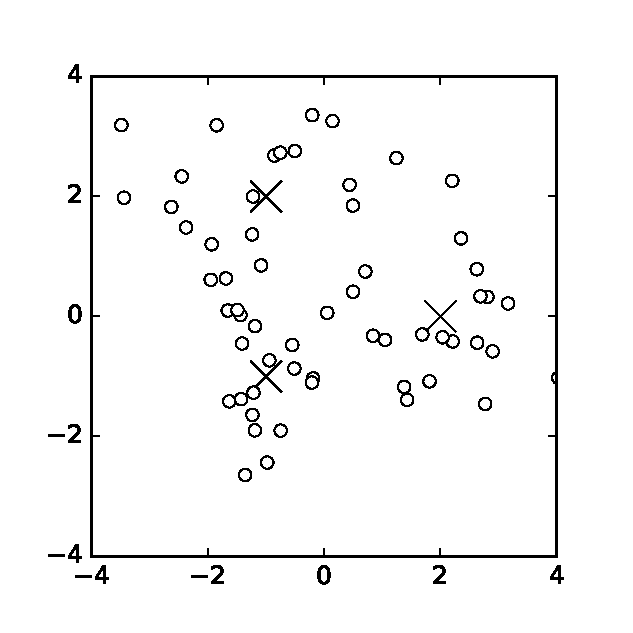
\includegraphics[width=\textwidth]{figures/denoising-noisy}
    \caption{Original samples}
    \label{fig:noisy}
  \end{subfigure}
  \hspace{1cm}
  \begin{subfigure}{0.3\textwidth}
    \centering
    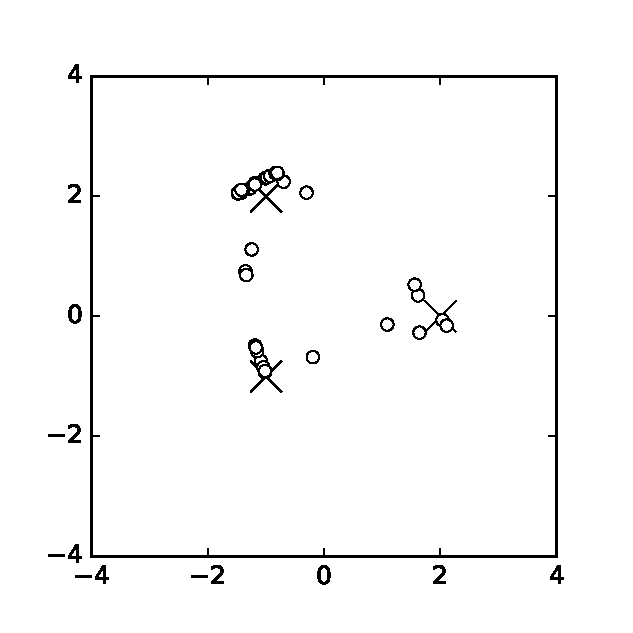
\includegraphics[width=\textwidth]{figures/denoising-denoised}
    \caption{After denoising}
    \label{fig:denoised}
  \end{subfigure}
  \caption{The samples have been tightly clustered and split into groups through denoising. The crosses mark the centers of three normal distributions while the circles denote samples.}
  \label{fig:denoising}
\end{figure}

In the second step called \emph{denoising} they define $P \in \mathbb{R}^{m \times N}$ as a matrix that has $x_{a, i}$ as its $(a, i)$-th column.
Then they argue that the matrix $PX_{R}$ has $\tilde{\gamma}_{a}$ as its $(a, i)$-th column and prove that the columns of $PX_{D}$ denoted by $c_{a, i}$ approximate the $\tilde{\gamma}_{a}$ as a consequence of the first step.
The $c_{a, i}$ are called the \emph{denoised data points}.
Figure \ref{fig:denoising} demonstrates the surprising effectiveness of this procedure by applying it to three Gaussians with $20$ samples each.

Lastly they perform the so called \emph{rounding}, an iterative algorithm that selects $k$ of the denoised data points as approximations to the $\tilde{\gamma}_{a}$, i.e. the k-means-optimal centroids.
During the implementation of the rounding algorithm we noticed that it requires the choice of an $\varepsilon$ to construct an intermediate graph structure.
Since this choice is the stimulus for our theory work in Section \ref{sec:epsilon}, we will now present the central rounding theorem from the paper and its proof.

\section{Selecting Cluster Center Approximations}
\label{sec:rounding}

\begin{theorem}
  \label{thm:rounding}
  Take $\varepsilon < \nicefrac{\Delta_{min}}{8}$, suppose
  \begin{equation*}
    \#\left\{ (a, i) : ||c_{a, i} - \tilde{\gamma}_{a}||_{2} > \varepsilon \right\} < \frac{n}{2}
  \end{equation*}
  and consider the graph $G$ of vertices $\{ c_{a, i} \}_{a = 1,}^{k}{}_{i = 1}^{n}$ such that $c_{a, i} \leftrightarrow c_{b, j}$ if $||c_{a, i} - c_{b, j}||_{2} \le 2\varepsilon$.
  For each $i = 1, \dots, k$ select the vertex $v_{i}$ of maximum degree (breaking ties arbitrarily) and update $G$ by removing every vertex $w$ such that $||w - v_{i}||_{2} \le 4\varepsilon$.
  Then there exists a permutation $\pi$ on $\{ 1, \dots, k \}$ such that
  \begin{equation*}
    ||v_{i} - \tilde{\gamma}_{\pi(i)}||_{2} \le 3\varepsilon
  \end{equation*}
  for every $i \in \{ 1, \dots, k \}$.
\end{theorem}

\begin{proof}
  We will prove the theorem by showing that a set of invariants holds across all $k$ iterations, one of which is the claim itself.
  Denote by $R_{i}$ the set of clusters for which we have not yet selected an approximation $v_{i}$, i.e. $R_{1} = \{ 1, \dots, k \}$ and $R_{i + 1} = R_{i} \setminus \{ \pi(i) \}$.
  Then the invariants read
  \begin{enumerate}[label=(\roman*)]
  \item \label{item:inv-outside} less than $\nicefrac{n}{2}$ vertices lie outside $\bigcup_{a \in R_{i}} B(\tilde{\gamma}_{a}, \varepsilon)$,
  \item \label{item:inv-inside} at least $\nicefrac{n}{2}$ vertices lie inside $B(v_{i}, 2\varepsilon)$ and
  \item \label{item:inv-unique} there exists a unique $a \in R_{i}$ such that $||v_{i} - \tilde{\gamma}_{a}||_{2} \le 3\varepsilon$
  \end{enumerate}
  where $B(x, r)$ is the closed ball around $x$ with radius $r$.
  First, we show that \ref{item:inv-outside} and \ref{item:inv-inside} imply \ref{item:inv-unique}.
  Afterwards we show by induction that \ref{item:inv-outside} and \ref{item:inv-inside} hold in every iteration and how to choose $\pi(i)$.

  From \ref{item:inv-outside} we know that there are at least $\nicefrac{n}{2}$ vertices in $B(v_{i}, 2\varepsilon)$.
  In combination with \ref{item:inv-inside} we get that at least one of them has to be in $B(\tilde{\gamma}_{a}, \varepsilon)$ for some $a \in R_{i}$ and thus $||v_{i} - \tilde{\gamma}_{a}||_{2} \le 3\varepsilon$ by the triangle inequality.
  Furthermore $3\varepsilon < \nicefrac{3}{8}\Delta_{min} < \nicefrac{\Delta_{min}}{2}$ making $a$ unique and we set $\pi(i) = a$ which gives us \ref{item:inv-unique}.

  In the first iteration \ref{item:inv-outside} is assumed and regarding \ref{item:inv-inside} we see that every ball $B(\tilde{\gamma}_{a}, \varepsilon)$ contains at least $\nicefrac{n}{2}$ vertices.
  Again using the triangle inequality we conclude that every vertex has a degree of at least $\nicefrac{n}{2} - 1$ and therefore at least $\nicefrac{n}{2}$ vertices in its $2\varepsilon$-ball.
  This is true in particular for the vertex of maximum degree, giving us \ref{item:inv-inside}.

  Assume \ref{item:inv-outside}, \ref{item:inv-inside} and \ref{item:inv-unique} for iteration $i < k$.
  Since $B(\tilde{\gamma}_{\pi(i)}, \varepsilon) \subset B(v_{i}, 4\varepsilon)$, the removal step removes all vertices inside $B(\tilde{\gamma}_{\pi(i)}, \varepsilon)$ and consequently ensures that \ref{item:inv-outside} holds for iteration $i + 1$.
  On top of this, if $v$ is a vertex to be removed, we have
  \begin{equation}
    ||v - \tilde{\gamma}_{\pi(i)}||_{2} \le ||v - v_{i}||_{2} + ||v_{i} - \tilde{\gamma}_{\pi(i)}||_{2} \le 7\varepsilon \label{eq:questionable}
  \end{equation}
  which implies that no vertices within an $\varepsilon$-radius of any other cluster center are removed.
  As a consequence invariant \ref{item:inv-inside} continues to hold in iteration $i + 1$ with the same argument as in the base case.
\end{proof}

This is how the proof is presented in the paper but on closer consideration the conclusion from Equation \eqref{eq:questionable} relies on the fact that $||\tilde{\gamma}_{a} - \tilde{\gamma}_{b}||_{2} > 8\varepsilon$ for all $a \ne b$.
Yet this might not be true because indeed $8\varepsilon < \Delta_{min} \le ||\gamma_{a} - \gamma_{b}||_{2}$ but this does not necessarily hold for the random variable $||\tilde{\gamma}_{a} - \tilde{\gamma}_{b}||_{2}$ which could take on values less than $\Delta_{min}$.

The rounding algorithm has two preconditions: first, you have to choose an $\varepsilon < \nicefrac{\Delta_{min}}{8}$ and second, less than $\nicefrac{n}{2}$ denoised data points are allowed to be farther than an $\varepsilon$ away from their respective k-means-optimal centroid.
The former requires an estimate of $\Delta_{min}$ (see Sec. \ref{sec:epsilon}) while the latter can be argued from the following denoising result shown in the paper.

\vspace{.5em}
\begin{theorem}
  Suppose $\sigma \utilde{<} \Delta_{min} / \sqrt{k}$. Then
  \begin{equation}
    \frac{1}{N} \sum_{a = 1}^{k} \sum_{i = 1}^{n} ||c_{a, i} - \tilde{\gamma}_{a}||_{2}^{2} \utilde{<} \frac{||\Gamma||_{2 \rightarrow 2}^{2}}{\Delta_{min}^{2}} \cdot k\sigma^{2}
    \label{eq:denoising-bound}
  \end{equation}
  with high probability as $n \rightarrow \infty$.
  Here, the $a$th column of $\Gamma$ is $\tilde{\gamma}_{a} - \frac{1}{k} \sum_{b = 1}^{k} \tilde{\gamma}_{b}$.
\end{theorem}

This means that the mean squared error of the denoised data points is bounded by $k\sigma^{2}$ with high probability if none of the cluster center approximators is too far away from their mean, which is equivalent to the condition that no cluster is too far out insofar that the $\tilde{\gamma}_{a}$ converge to the true $\gamma_{a}$.
Taking the square root on both sides of Equation \eqref{eq:denoising-bound}, we get
\begin{equation*}
  \frac{1}{\sqrt{N}} \sqrt{\sum_{a = 1}^{k} \sum_{i = 1}^{n} ||c_{a, i} - \tilde{\gamma}_{a}||_{2}^{2}} \utilde{<} \sqrt{k} \sigma \utilde{<} \Delta_{min}.
\end{equation*}
A further application of Jensen's inequality for concave functions and dividing both sides by $\sqrt{N}$ yields
\begin{equation}
  \frac{1}{N} \sum_{a = 1}^{k} \sum_{i = 1}^{n} ||c_{a, i} - \tilde{\gamma}_{a}||_{2} \utilde{<} \frac{\Delta_{min}}{\sqrt{N}}.
  \label{eq:mean-error-bound}
\end{equation}
We see that the mean distance between $c_{a, i}$ and the associated $\tilde{\gamma}_{a}$ is bounded by $\nicefrac{\Delta_{min}}{\sqrt{N}}$.
Consequently there will be few denoised data points with $||c_{a, i} - \tilde{\gamma}_{a}||_{2} > \varepsilon$ for some $\varepsilon < \nicefrac{\Delta_{min}}{8}$ -- in particular less than $\nicefrac{n}{2}$ for $N$ large enough -- justifying the second precondition.
The following sketch shows that $N \in O(k^{2})$ data points suffice.
Let $p$ be the number of denoised data points with a distance $||c_{a, i} - \tilde{\gamma}_{a}||_{2}$ of at least $\varepsilon$.
Since all distances are non-negative, $p$ is maximized if the distances are minimized, i.e. $p$ points have a distance of $\varepsilon$ and the rest has a distance of $0$.
Assume that $\varepsilon$ is chosen not too small, i.e. $\nicefrac{\Delta_{min}}{\varepsilon} \le q$ for some $q > 8$.
\begin{equation*}
  \frac{1}{N} \cdot p \cdot \varepsilon \utilde{<} \frac{\Delta_{min}}{\sqrt{N}} \Leftrightarrow p \utilde{<} \frac{\Delta_{min}}{\varepsilon} \sqrt{N} < q \sqrt{N}
\end{equation*}
Now we can compute a lower bound for $N$ by checking when the upper bound is less than $\nicefrac{n}{2}$.
\begin{equation*}
  q \sqrt{N} = q \sqrt{kn} < \frac{n}{2} \Leftrightarrow (2q)^{2}k < n \Leftrightarrow N > (2q)^{2} k^{2} > 256k^{2}
\end{equation*}
This shows first that $N \in O(k^{2})$ data points suffice to satisfy the second condition of Theorem \ref{thm:rounding} and second that you want to choose an $\varepsilon$ as close to $\nicefrac{\Delta_{min}}{8}$ as possible to require fewer data points.

\section{Choosing an $\varepsilon$}
\label{sec:epsilon}

In the previous section we have seen that the rounding step presented in Theorem \ref{thm:rounding} requires the choice of an $\varepsilon$.
On the one hand the choice has to respect an upper bound of $\nicefrac{\Delta_{min}}{8}$ and on the other hand you want to pick a value as large as possible.
In the optimal case one would chose something similar to $\varepsilon = \nicefrac{\Delta_{min}}{9}$ but a priori this is infeasible because $\Delta_{min}$ is unknown.
Consequently its value has to be estimated from the data.

\begin{figure}[h]
  \centering
  \includegraphics[width=\textwidth]{figures/chessboard}
  \caption{$\log_{10}$ of the exact solution $X_{R}$, the relaxation solution $X_{D}$ for a stochastic ball model and the relaxation solution $X_{D}$ of a mixture of normals model}
  \label{fig:chessboard}
\end{figure}

Figure \ref{fig:chessboard} presents matrix plots of solutions $X$ of the SDP in the following two settings.
In both cases there are three clusters centered at $(-2, -1), (-1, 2.5), (3, 1)$ with $10$, $15$ and $15$ samples.
The difference is that the first setting uses stochastic ball models of radii $1$, $1$ and $1.5$ while the second setting uses multivariate normal distributions of variance $1$, $1$ and $1.5$.
All plots actually show the element-wise $\log_{10}$ to make the noise visible.
The first two plots are from the stochastic ball scenario whereas the former shows the exact solution $X$ as defined in the introduction as cluster-affinity matrix while the latter shows the solution $X_{D}$ as computed by our implementation.
The last plot on the right again shows the minimizer of the SDP but for the mixture of normals model.

The exact solution has non-zero block matrices on the diagonal and is zero everywhere else which allows for an easy recovery of the cluster affinities.
Even though the center matrix is non-zero everywhere it is still basically the exact solution with some very light noise on the order of $10^{-9}$ applied.
As we will see shortly you can recover the cluster affinities from this noisy result just as well as from the exact solution.
The last case is the most interesting as the unboundedness of the normal distribution has introduced as significant deviation from the optimal solution.
Nonetheless you can still recognize the block structure and at least experimentally we have seen that this is good enough for a working estimate of $\Delta_{min}$.

From these observations we have defined the following greedy algorithm to perform this estimate.

\vspace{0.5em}
\begin{algorithm}
  \label{alg:d-min}
  Let $X_{D}$ be the minimizer of the SDP.
  Furthermore define $C = \{ 1, \dots, N \}$ as the set of nodes which have not been assigned to a cluster yet and let $i = 1$ be the cluster that we are currently assigning nodes to.
  \begin{enumerate}[label=(\roman*)]
  \item \label{item:clusters} Repeat until $C = \emptyset$
    \begin{enumerate}
    \item Select $j \in C$
    \item Define $C_{i} = \{ j' : j' \in C\ \text{and}\ X_{D,jj'} \ge \frac{1}{N} \}$
    \item Update $C \leftarrow C \setminus C_{i}$ and $i \leftarrow i + 1$
    \end{enumerate}
  \item \label{item:gamma-hat} Compute $\hat{\Gamma} = \left\{ \frac{1}{|C_{j}|} \sum_{j' \in C_{j}} x_{j'} : j \in \{ 1, \dots, i - 1 \} \right\}$
  \item \label{item:d-min} Estimate $\Delta_{min}$ by $\tilde{\Delta}_{min} = \min_{a \ne b} ||\hat{\Gamma}_{a} - \hat{\Gamma}_{b}||_{2}$
  \end{enumerate}
\end{algorithm}

In the first step we reconstruct the clusters $C_{i}$ from $X_{D}$ by selecting rows of $X_{D}$ and assigning all points to the same cluster whose column value in the respective row is at least $\nicefrac{1}{N}$ until all points have been assigned.
The choice of lower bound is based on the fact that it is the smallest non-zero value that an entry can assume in the exact solution.
The second step computes the means $\hat{\Gamma}$ from the recovered clusters.
For the rest of this section we denote the elements of $\hat{\Gamma}$ by $\hat{\gamma}_{i}$.
Finally step \ref{item:d-min} estimates $\Delta_{min}$ by computing the minimum distance between any pair of $\hat{\gamma}_{i}$.

The following lemma shows that Algorithm \ref{alg:d-min} recovers the cluster affinities from the exact solution and from the minimizer for stochastic ball models as long as they are sufficiently far separated, since the noise decreases with larger separation.

\vspace{0.5em}
\begin{lemma}
  \label{lemma:noise}
  Let $\varepsilon_{max} = \max_{i,j} |X_{D,ij} - X_{ij}|$, where $X_{D}$ is the minimizer of the SDP and $X$ is the exact solution, be the maximum noise.
  Furthermore let $A_{1}, \dots, A_{k}$ be the optimal cluster assignments as defined in the original problem.
  If $\varepsilon_{max} \le \min_{i \in [k]} \nicefrac{1}{|A_{i}|} - \nicefrac{1}{N}$ and $\varepsilon_{max} < \nicefrac{1}{N}$, Algorithm \ref{alg:d-min} will reconstruct the clusters as given by $A_{1}, \dots, A_{k}$.
\end{lemma}

\begin{proof}
  Select some row $i$ and consider its $j$th column.
  Let $t \in [k]$ such that $i \in A_{t}$.
  The algorithm will put $i$ and $j$ into the same cluster iff $X_{D,ij} \ge \nicefrac{1}{N}$.
  Consider the following two cases.
  In the first case $j \not\in A_{t}$ but $X_{D,ij} \ge \nicefrac{1}{N}$.
  Since $i$ and $j$ do not belong to the same cluster, we know that $X_{ij} = 0$ from which it follows that $|X_{D,ij} - X_{ij}| \ge \nicefrac{1}{N}$ contradicting the precondition.
  In the second case $j \in A_{t}$ but $X_{D,ij} < \nicefrac{1}{N}$.
  From the definition of $X$ we know that $X_{ij} = \nicefrac{1}{|A_{t}|}$ yielding
  \begin{equation*}
    |X_{D,ij} - X_{ij}| = X_{ij} - X_{D,ij} > \frac{1}{|A_{t}|} - \frac{1}{N} \ge \min_{i \in [k]} \frac{1}{|A_{i}|} - \frac{1}{N}
  \end{equation*}
  which again contradicts the precondition.
  In combination this means that $j \in A_{t} \Leftrightarrow j \in C_{t'}$ where $t' \in [k]$ such that $i \in C_{t'}$ which shows that the algorithm finds the original $A_{1}, \dots, A_{k}$.
\end{proof}

Step \ref{item:d-min} of the algorithm produces the estimate $\tilde{\Delta}_{min} = \min_{a, b} ||\hat{\gamma}_{a} - \hat{\gamma}_{b}||_{2}$.
As we have just seen this is actually equal to $||\tilde{\gamma}_{a} - \tilde{\gamma}_{b}||_{2}$ in the case of stochastic ball models under the preconditions of Lemma \ref{lemma:noise}.
In the following analysis we will restrict ourselves to these models though the experiments in Section \ref{sec:results} indicate that the algorithm also works in a more general setting.
In the rest of this section we will show that our estimator will not be too large compared to $\Delta_{min}$ with high probability by using the following theorem from Tropp's paper \cite{tailbounds} on tail bounds for sums of random matrices.

\vspace{.5em}
\begin{theorem}[Matrix Bernstein]
  \label{thm:matrix-bernstein}
  Consider a finite sequence $\{ X_{k} \}$ of independent, random, self-adjoint matrices with dimension $d$.
  Assume that each random matrix satisfies
  \begin{equation*}
    \mathbb{E}\,X_{k} = 0 \quad \text{and} \quad \lambda_{max}(X_{k}) \le R\ \text{almost surely.}
  \end{equation*}
  Then, for all $\delta \ge 0$,
  \begin{equation*}
    \mathbb{P}\left( \lambda_{max}\left( \sum_{k} X_{k} \right) \ge \delta \right) \le d \cdot \exp\left( -\frac{\nicefrac{\delta^{2}}{2}}{\sigma^{2} + R \nicefrac{\delta}{3}} \right)
  \end{equation*}
  where $\sigma^{2} = ||\sum_{k} \mathbb{E}\,X_{k}^{2}||$.
\end{theorem}

First, we are going to see that the estimators $\tilde{\gamma}_{t}$ are concentrated around their respective means $\gamma_{t}$.
In the following we will use $x_{t, l}$ as random variables with distribution $\mathcal{D}_{t}$ instead of the concrete samples.
Since we restricted ourselves to stochastic ball models, we can safely assume that $||x_{t, l} - \gamma_{t}||_{2} \le R_{t}$ for some $R_{t} > 0$.

\vspace{.5em}
\begin{lemma}
  \label{lemma:concentration}
  If there exists an $R_{t} > 0$ for each $t \in [k]$ such that $||X_{t, l} - \gamma_{t}||_{2} \le R_{t}$ for all $l \in [n_{t}]$, then, for all $\delta \ge 0$,
  \begin{equation*}
    \mathbb{P}\left( ||\tilde{\gamma}_{t} - \gamma_{t}||_{2} \ge \delta \right) \le (m + 1) \cdot \exp\left( -\frac{\delta^{2} \nicefrac{n_{t}}{2}}{R_{t} \nicefrac{\delta}{3} + \sum_{l = 1}^{m} \sigma_{t, l}^{2}} \right).
  \end{equation*}
\end{lemma}

\begin{proof}
  Define random variables $y_{l} = x_{t, l} - \gamma_{t}$ and random, self-adjoint matrices
  \begin{equation*}
    Y_{l} = \begin{pmatrix}
      0 & y_{l}^{T}\\
      y_{l} & 0
    \end{pmatrix}.
  \end{equation*}
  Since the $y_{l}$ are independent and $\mathbb{E}\,y_{l} = 0$, the matrices $Y_{l}$ are independent with $\mathbb{E}\,Y_{l} = 0$ and $\lambda_{max}(Y_{l}) = ||y_{l}||_{2}$.
  The second property follows from the form of $Y_{l}Y_{l}^{T} = Y_{l}^{2}$ computed in Equation \eqref{eq:y-t-squared} and the fact that the singular values are the square roots of the eigenvalues of $Y_{l}^{2}$.
  It is of rank $2$ and has two eigenvalues both of which are $||y_{l}||_{2}^{2}$ (the corresponding eigenvectors are $e_{1}$ and $(0, y_{l})$).
  Applying theorem \ref{thm:matrix-bernstein} we can derive
  \begin{align*}
    \mathbb{P}(||\tilde{\gamma}_{t} - \gamma_{t}||_{2} \ge \delta) & = \mathbb{P}\left( \frac{1}{n_{t}} \left|\left| \sum_{l = 1}^{n_{t}} x_{t, l} - \gamma_{t} \right|\right|_{2} \ge \delta \right) = \mathbb{P}\left( \left|\left| \sum_{l = 1}^{n_{t}} y_{l} \right|\right|_{2} \ge n_{t}\delta \right)\\
    & = \mathbb{P}\left( \lambda_{max}\left( \sum_{l = 1}^{n_{t}} Y_{l} \right) \ge n_{t}\delta \right) \le (m + 1) \cdot \exp\left( -\frac{\delta^{2} \nicefrac{n_{t}^{2}}{2}}{R_{t} \nicefrac{\delta n_{t}}{3} + \sigma^{2}} \right)
  \end{align*}
  with $\sigma^{2} = \left|\left| \sum_{l} \mathbb{E}\, Y_{l}^{2} \right|\right|$.
  To determine $\sigma^{2}$, i.e. the largest singular value of $\sum_{l} \mathbb{E}\,Y_{l}^{2}$, we will first determine the actual form of the sum terms.
  \begin{equation}
    \mathbb{E}\,Y_{l}^{2} = \mathbb{E}\,\begin{pmatrix}
      y_{l}^{T}y_{l} & 0\\
      0 & y_{l}y_{l}^{T}
    \end{pmatrix}
    = \begin{pmatrix}
      \Tr(\Sigma_{t}) & 0\\
      0 & \Sigma_{t}
    \end{pmatrix}
    \label{eq:y-t-squared}
  \end{equation}
  Now let $UWV^{*}$ be a singular value decomposition of $\Sigma_{t}$.
  Then we can write $\mathbb{E}\,Y_{l}$ as
  \begin{equation*}
    \mathbb{E}\,Y_{l}^{2} = \begin{pmatrix}
      1 & 0\\
      0 & U
    \end{pmatrix}
    \begin{pmatrix}
      \Tr(\Sigma_{t}) & 0\\
      0 & W
    \end{pmatrix}
    \begin{pmatrix}
      1 & 0\\
      0 & V^{*}
    \end{pmatrix}.
  \end{equation*}
  Since the left- and right-hand matrix are unitary and the matrix in the center is diagonal, this form is a singular value decomposition of $\mathbb{E}\,Y_{l}$ and the center matrix's diagonal carries the singular values.
  Therefore the maximum singular value of $\mathbb{E}\,Y_{l}^{2}$ is
  \begin{equation*}
    ||\mathbb{E}\,Y_{l}^{2}|| = \max\left( \Tr(\Sigma_{t}), \lambda_{max}(\Sigma_{t}) \right) = \max\left( \sum_{l = 1}^{m} \sigma_{t, l}^{2}, \sigma_{t, m}^{2} \right) = \sum_{l = 1}^{m} \sigma_{t, l}^{2}.
  \end{equation*}
  In combination with
  \begin{equation*}
    \sigma^{2} = \left|\left| \sum_{l = 1}^{n_{t}} \mathbb{E}\,Y_{l}^{2} \right|\right| = n_{t} \left|\left| \mathbb{E}\,Y_{1}^{2} \right|\right|
  \end{equation*}
  we obtain the claimed result.
\end{proof}

Finally we will apply this intermediate result to show that the estimate $\tilde{\Delta}_{min} = \min_{s, t} ||\tilde{\gamma}_{s} - \tilde{\gamma}_{t}||_{2}$ is not too large with high probability.

\vspace{.5em}
\begin{lemma}
  \label{lemma:bound}
  Let $a, b$ be the minimizers of $\min_{\substack{a, b\\a \ne b}} ||\gamma_{a} - \gamma_{b}||_{2}$.
  Then
  \begin{equation*}
    \mathbb{P}\left( \min_{\substack{s, t\\s \ne t}} ||\tilde{\gamma}_{s} - \tilde{\gamma}_{t}||_{2} - \Delta_{min} \ge \delta \right) \le (m + 1) \begin{pmatrix} \exp\left( -\frac{\delta^{2} \nicefrac{n_{a}}{8}}{R_{a} \nicefrac{\delta}{6} + \sum_{k = 1}^{m} \sigma_{a,k}^{2}} \right)\\ + \exp\left( -\frac{\delta^{2} \nicefrac{n_{b}}{8}}{R_{b} \nicefrac{\delta}{6} + \sum_{k = 1}^{m} \sigma_{b,k}^{2}} \right) \end{pmatrix}
  \end{equation*}
\end{lemma}

\begin{proof}
  The first step is to see that the difference between our estimator and $\Delta_{min}$ can be upper-bounded by the distance between the k-means-optimal centroids of clusters $a$ and $b$ and their respective true centers.
  \begin{align*}
    \min_{\substack{s, t\\s \ne t}} ||\tilde{\gamma}_{s} - \tilde{\gamma}_{t}||_{2} - \Delta_{min} & = \min_{\substack{s, t\\s \ne t}} ||\tilde{\gamma}_{s} - \tilde{\gamma}_{t}||_{2} - \min_{\substack{c, d\\c \ne d}} ||\gamma_{c} - \gamma_{d}||_{2}\\
    \intertext{The minimum is surely less than the distance between two specific $\tilde{\gamma}.$}
    & \le ||\tilde{\gamma}_{a} - \tilde{\gamma}_{b}||_{2} - ||\gamma_{a} - \gamma_{b}||_{2}\\
    & = ||\tilde{\gamma}_{a} - \gamma_{a} + \gamma_{a} - \gamma_{b} + \gamma_{b} - \tilde{\gamma}_{b}||_{2} - ||\gamma_{a} - \gamma_{b}||_{2}\\
    & \le ||\tilde{\gamma}_{a} - \gamma_{a}||_{2} + ||\tilde{\gamma}_{b} - \gamma_{b}||_{2} & \text{Triangle inequality}
  \end{align*}

  In a second step we can use this upper bound and the concentration inequality from Lemma \ref{lemma:concentration} to in turn give an upper bound on the probability that $\tilde{\Delta}_{min}$ is larger than $\Delta_{min} + \delta$ for some $\delta \ge 0$.
  \begin{align*}
    \mathbb{P}\left( \min_{\substack{s, t\\s \ne t}} ||\tilde{\gamma}_{s} - \tilde{\gamma}_{t}||_{2} - \Delta_{min} \ge \delta \right) & \le \mathbb{P}\left( ||\tilde{\gamma}_{a} - \gamma_{a}||_{2} + ||\tilde{\gamma}_{b} - \gamma_{b}||_{2} \ge \delta \right)\\
    \intertext{If the sum of the distances is greater than or equal to $\delta$, at least one of them has to be greater than or equal to $\nicefrac{\delta}{2}$.
    Therefore the previous event is included in the next one.}
    & \le \mathbb{P}\left( \max \left\{ ||\tilde{\gamma}_{a} - \gamma_{a}||_{2}, ||\tilde{\gamma}_{b} - \gamma_{b}||_{2} \right\} \ge \frac{\delta}{2} \right)\\
    & \le \mathbb{P}\left( ||\tilde{\gamma}_{a} - \gamma_{a}||_{2} \ge \frac{\delta}{2} \right) + \mathbb{P}\left( ||\tilde{\gamma}_{b} - \gamma_{b}||_{2} \ge \frac{\delta}{2} \right) & \text{Union bound}\\
    & \le (m + 1) \begin{pmatrix} \exp\left( -\frac{\delta^{2} \nicefrac{n_{a}}{8}}{R_{a} \nicefrac{\delta}{6} + \sum_{k = 1}^{m} \sigma_{a,k}^{2}} \right)\\ + \exp\left( -\frac{\delta^{2} \nicefrac{n_{b}}{8}}{R_{b} \nicefrac{\delta}{6} + \sum_{k = 1}^{m} \sigma_{b,k}^{2}} \right) \end{pmatrix} & \text{Lemma \ref{lemma:concentration}}
  \end{align*}
\end{proof}

In the end we come to the actual choice of $\varepsilon$.
For this we will assume that all clusters have at least $n_{min}$ samples, a maximum radius of $R_{max}$ and that $\sum_{k = 1}^{m} \sigma_{a,k}^{2}$ is bounded by some $\Sigma_{max}^{2}$ for all $a \in [k]$.
This lets us further simplify the upper bound from Lemma \ref{lemma:bound} to
\begin{equation*}
  2(m + 1)\exp\left( -\frac{\delta^{2} \nicefrac{n_{min}}{8}}{R_{max} \nicefrac{\delta}{6} + \Sigma_{max}^{2}} \right).
\end{equation*}
Setting this less than or equal to some $0 < \kappa \le 1$ and solving for $\delta$ yields
\begin{equation}
  \delta^{2} + \frac{8R_{max}}{6n_{min}}\log\left( \frac{\kappa}{2(m + 1)} \right)\delta \ge -\log\left( \frac{\kappa}{2(m + 1)} \right)\frac{8}{n_{min}}\Sigma_{max}^{2}.
  \label{eq:delta-epsilon}
\end{equation}
Since $\kappa$ is surely less than $2(m + 1)$, the right-hand side is a positive number and the left is an upwards opening parabola.
So in theory you could use Equation \eqref{eq:delta-epsilon} to determine a $\delta > 0$ such that $\mathbb{P}(\tilde{\Delta}_{min} - \Delta_{min} \ge \delta) \le \kappa$ and set $\varepsilon = \nicefrac{\tilde{\Delta}_{min} - \delta}{8}$ which would be less than $\nicefrac{\Delta_{min}}{8}$ with probability $\kappa$.
In practice however it is impossible because all values besides $\kappa$ and $m$ are unknown.

It is also quite possible that our bounds are far from tight, since this formula applied to the scenario in Figure \ref{fig:chessboard} results in $\delta \approx 3.2$.
This in turn would result in a choice of $\varepsilon$ very close to $0$ and possibly even negative, even though choices of $\varepsilon$ up to $0.45$ would be valid.
Therefore we decided to run all our experiments in the next section with $\varepsilon = \nicefrac{\tilde{\Delta}_{min}}{10}$.

\section{An Implementation}
\label{sec:results}

We have implemented the complete algorithm including the estimation of $\Delta_{min}$ as a python program.
It is built on top of \texttt{scipy}/\texttt{numpy} for easy handling of matrices and uses \texttt{picos} and \texttt{cvxopt} to solve the SDP and \texttt{networkx} for graph operations, for example extracting the node of maximum degree.
The code is available for inspection and hosted on github\footnote{\url{https://github.com/cqql/tum-cs/tree/master/idp/src}}.
In the following we will present different clustering results to showcase the performance of the algorithm.
Each of the Figures \ref{fig:results-balls} to \ref{fig:results-mixed-top} consists of three plots: the first shows just the samples, the second shows the denoised data points and the last one shows the k-means-optimal centroid marked with a triangle and the estimator that our algorithm selected as a star.
On top of that all plots include the true cluster centers that we are trying to approximate as crosses.

As expected one gets very good results in the case of non-overlapping stochastic ball models (Figure \ref{fig:results-balls}).
The approximations $v_{a}$ are close to the k-means-optimal centroids which in turn approximate the true centers well.
A slight error arises from the small distance between the left two clusters.
Figure \ref{fig:results-normals} shows the exact same situation but with normal distributions instead which have the former radii as their covariance.
It stands out that the denoising procedure could not fully separate the data points sampled from the left two clusters.
Consequently the estimators are also noticeably further off.
Lastly, Figure \ref{fig:results-mixed} demonstrates the case of mixed distributions with non-isotropic covariance.
The bottom two clusters are normal distributions and the top one is a stochastic ball model.
In addition the left-most cluster has a non-isotropic distribution where the variance in y-direction is twice as large as the variance in x-direction.
Also the number of samples drawn from it is twice the number of samples drawn from each of the other two clusters.
This time the denoising step has even more problems separating the data points which leads to an increased approximation error.
Yet it is still well within the bounds given by the performance guarantee in the paper.

\begin{figure}[h]
  \centering
  \begin{tabular}{c|c|c|c|c|c}
    Problem & Iterations & $\varepsilon$ & Misclassification rate & Total distance to $\gamma_{a}$ & Total distance to $\tilde{\gamma}_{a}$ \\
    \hline
    Figure \ref{fig:results-balls} & 1 & $0.308$ & 2\% & $0.639$ & $0.232$\\
    Figure \ref{fig:results-normals} & 1 & $0.28$ & 11\% & $1.444$ & $0.805$\\
    Figure \ref{fig:results-normals-iterated} & 2 & $0.279$ & 9\% & $1.021$ & $0.424$\\
    Figure \ref{fig:results-mixed} & 1 & $0.228$ & 20\% & $1.295$ & $1.266$\\
    Figure \ref{fig:results-mixed-iterated} & 3 & $0.232$ & 13\% & $0.873$ & $0.678$
  \end{tabular}
  \caption{Summary of result statistics of the different experiments. The misclassification rate refers to the classification/assignment step in Algorithm \ref{alg:d-min}.}
  \label{fig:results}
\end{figure}

\begin{figure}[h]
  \centering
  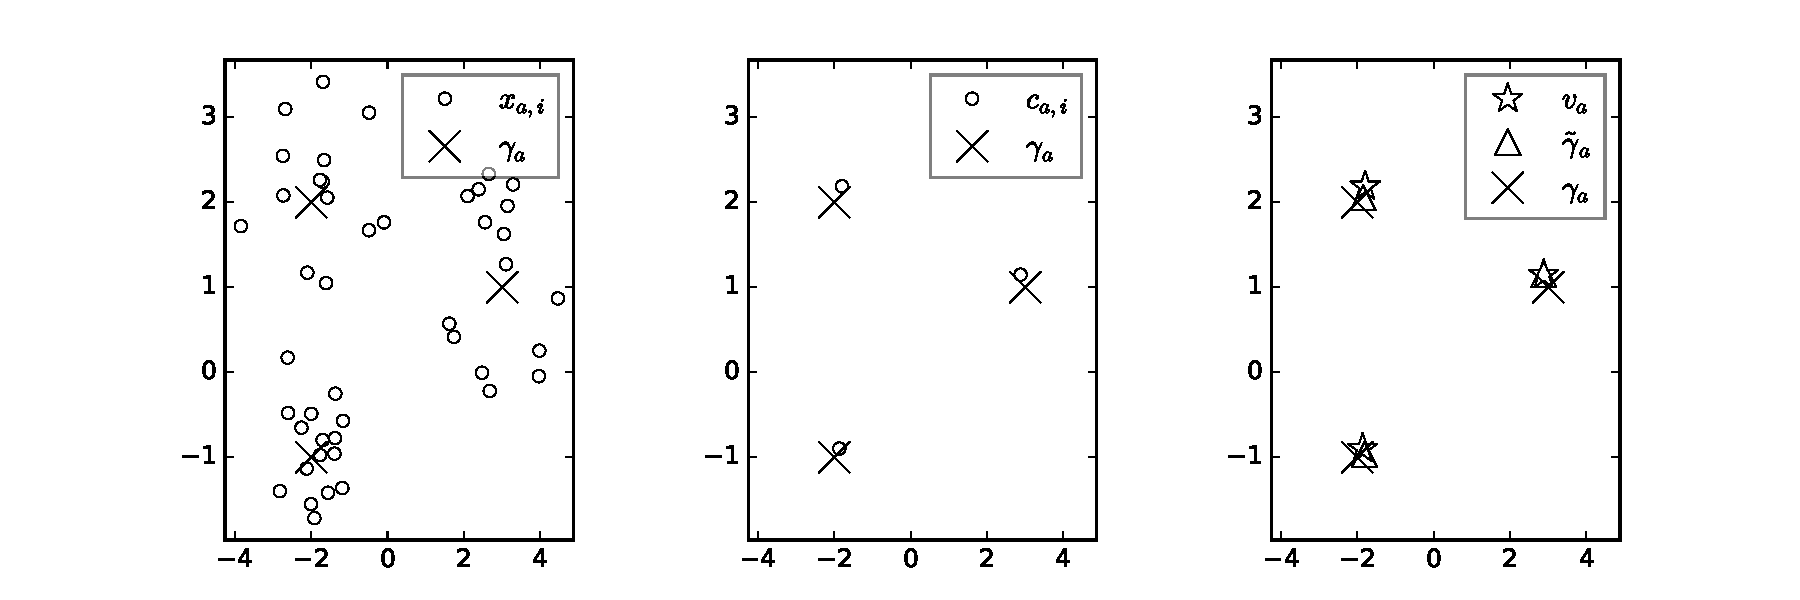
\includegraphics[width=\textwidth]{figures/results-3sb}
  \caption{3 non-overlapping stochastic ball model clusters}
  \label{fig:results-balls}
\end{figure}

\begin{figure}[h]
  \centering
  \begin{subfigure}{\textwidth}
    \centering
    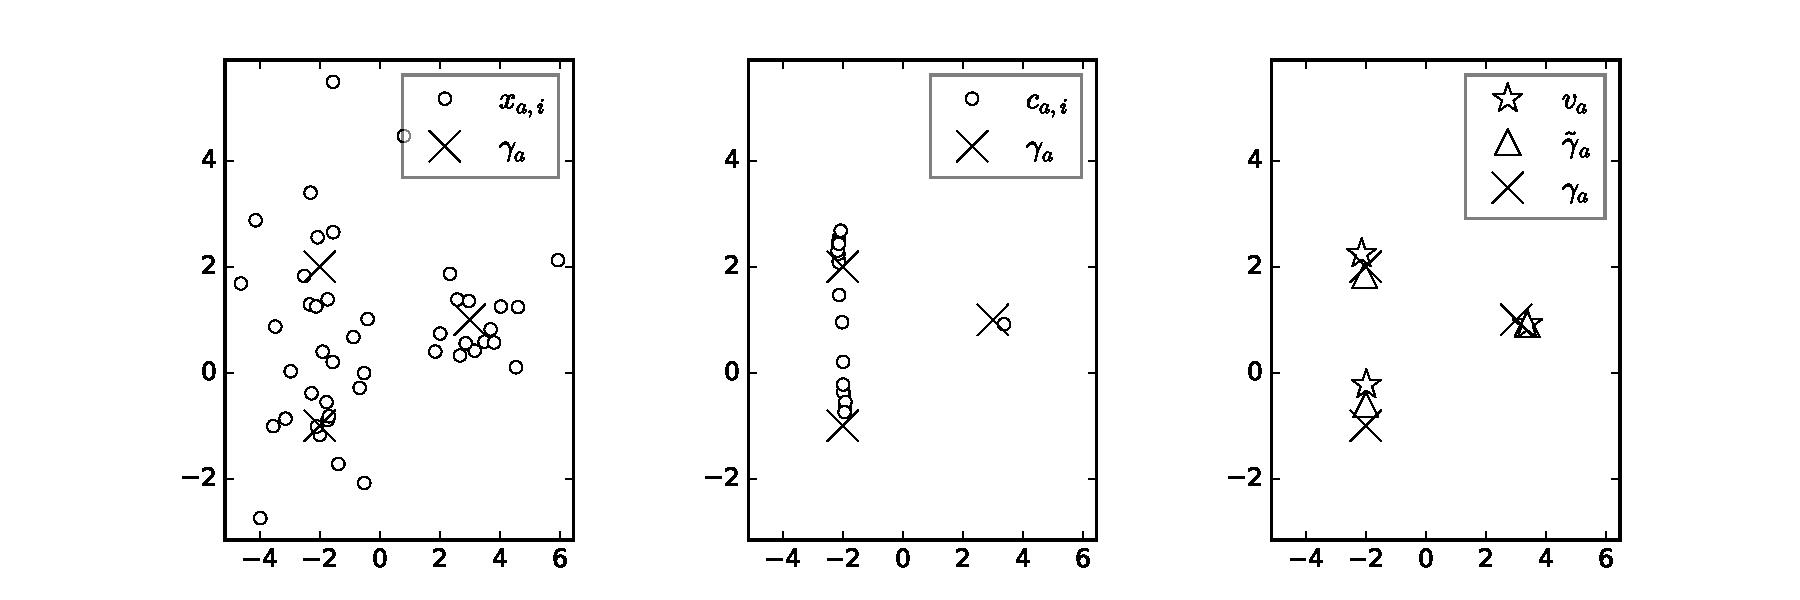
\includegraphics[width=\textwidth]{figures/results-3nm}
    \caption{Direct application of the algorithm}
\label{fig:results-normals}
  \end{subfigure}
  \begin{subfigure}{\textwidth}
    \centering
    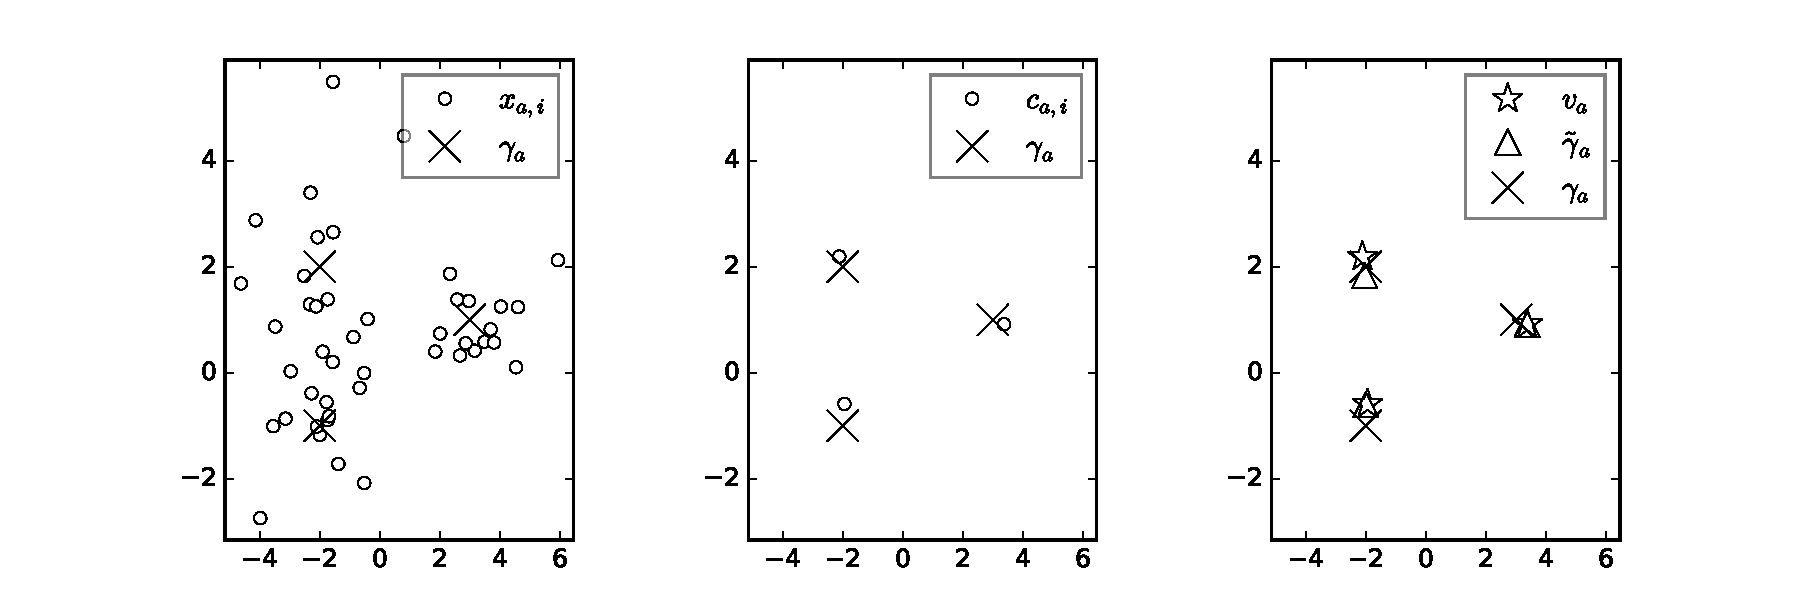
\includegraphics[width=\textwidth]{figures/results-3nm-iterated}
    \caption{A run with a second denoising step}
\label{fig:results-normals-iterated}
  \end{subfigure}
  \caption{3 clusters with identical, isotropic normal distributions}
\end{figure}

\begin{figure}[h]
  \centering
  \begin{subfigure}{\textwidth}
    \centering
    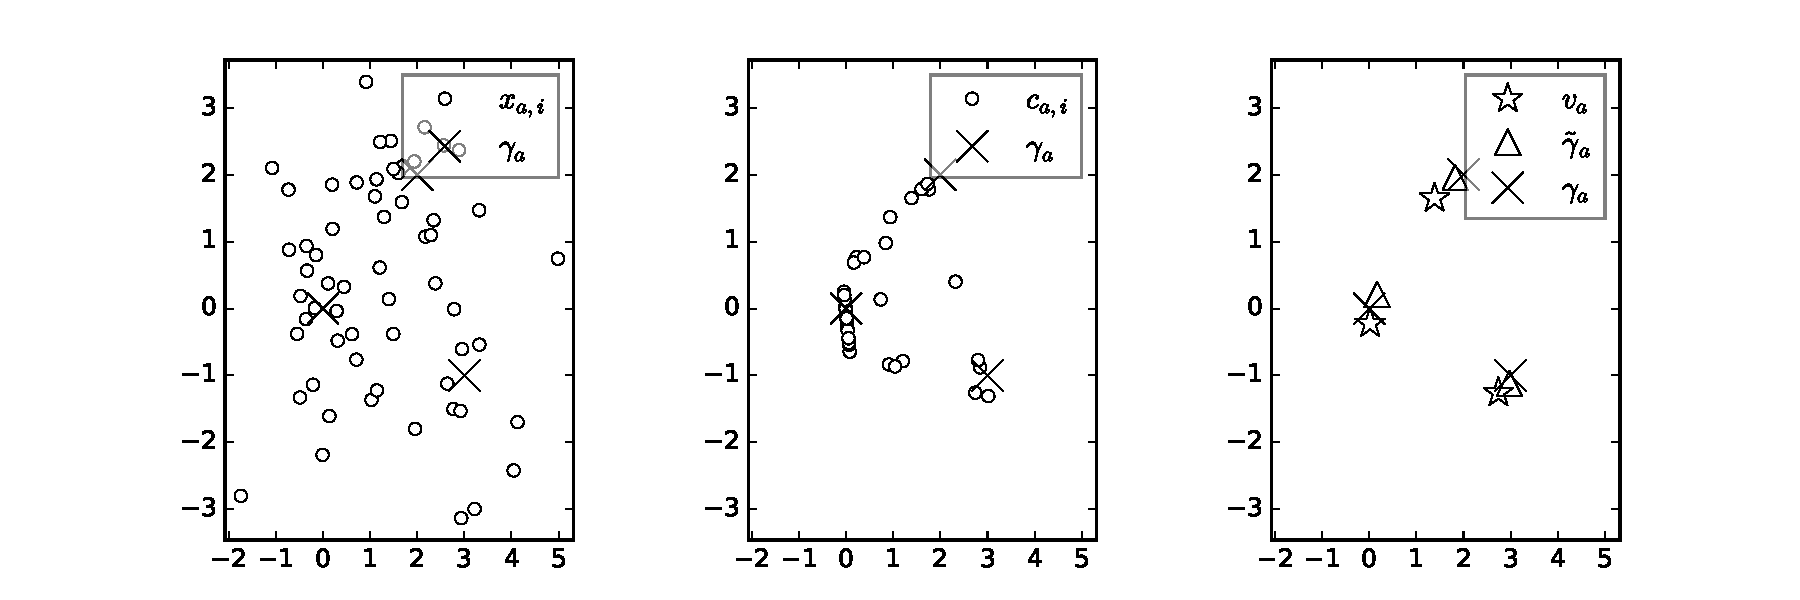
\includegraphics[width=\textwidth]{figures/results-mixed}
    \caption{Direct application of the algorithm}
\label{fig:results-mixed}
  \end{subfigure}
  \begin{subfigure}{\textwidth}
    \centering
    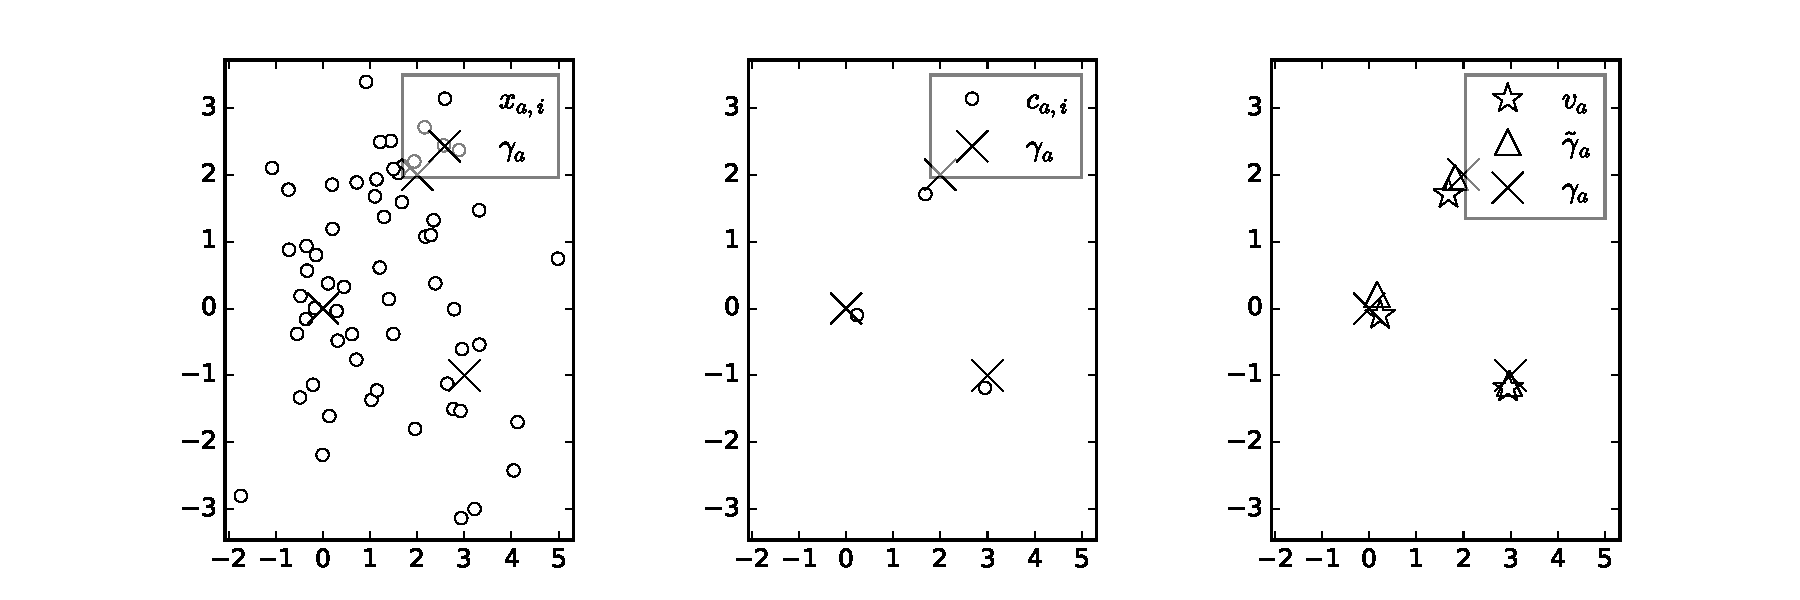
\includegraphics[width=\textwidth]{figures/results-mixed-iterated}
    \caption{It took three iterations of denoising to cluster the points that tightly}
\label{fig:results-mixed-iterated}
  \end{subfigure}
  \caption{3 clusters with different, non-isotropic distributions and differing numbers of samples drawn}
  \label{fig:results-mixed-top}
\end{figure}

During the project presentation Michael Sandbichler proposed the idea of iterating the denoising step.
The results can be found in Figure \ref{fig:results-normals-iterated}, \ref{fig:results-mixed-iterated} and Table \ref{fig:results}.
Surprisingly, it actually works and improves the approximation.
Enough iterations of denoising cluster the data points just as tightly as a single iteration does in the case of stochastic ball models.
At first we suspected that the second and later iterations might denoise the data even more but in a way that does not change or improve the performance in the end.
However, the statistics in Table \ref{fig:results} disprove that.
Actually the improvement is impressive and halved total error in both cases.

\section{Conclusion}
\label{sec:conclusion}

For me it was the first time working with an exact clustering algorithm.
Prior to this project I had only encountered the standard k-means algorithm and EM, both of which are heuristic.
Thus, it came as an exciting surprise to me how well these methods are working, even though they have nothing in common with the ones I knew before.
At the same time though I got the impression that SDP based clustering methods are basically not applicable to large problems because of the scaling behavior of SDP solvers.
The one I used was so slow that it could not even solve instances with $100$ data points in a reasonable time frame.
Of course other solvers might perform better and the paper authors solved a problem with $300$ data points in just 16 seconds but I suspect that their solver has the same scaling behavior up to constant factors.

The analysis in Section \ref{sec:epsilon} has two major points that one could improve.
First, one should try to find a tighter upper-bound so that the theoretical results achieve practical relevance.
A first step in this direction might be to switch out the Matrix Bernstein theorem for the Matrix Hoeffding theorem from the same paper \cite{tailbounds} which usually gives better results and has the added benefit of not including the radius $R$.
This leads over to the second point, the restriction to stochastic ball models.
One should be able to generalize this relatively easily to general subgaussian distributions by truncation.
That means that you transform the general distributions into bounded distributions by defining a cut-off distance from its center such that the probability weight outside of this inner ball is very small.
The outer probability mass is then counted towards the error probability while the inner probability mass defines the probability density of new, bounded random variables (after rescaling).

Finally I think that the idea of iterated denoising is interesting and worthy of further investigation, by experimentation as well as theoretically.

\bibliography{report}{}
\bibliographystyle{plain}

\end{document}
